%!TEX root = ../slides.tex

\section[eDSL for the SDR]{Embedded Domain Specific Language for the Software-defined Radio}

\subsection[Existing Solutions]{Existing Solutions}

\subsection[Proposed eDSL]{Description of the Proposed Embedded Domain Specific Language}

\begin{frame}{Motivations}
  % \vfill
  \begin{itemize}
    \item Need for environment adapted to SDR systems description
    \vspace{0.1cm}
    \item<2-> Existing solutions:
    \begin{itemize}
      \item Dedicated languages~\cite{Amarasinghe2005,DeOliveiraCastro2017} based on the \textbf{dataflow model}
      \item GNU Radio~\cite{GNURadio}
    \end{itemize}
    \vspace{0.1cm}
    % \pause
    % \item Objectives:
    % \begin{itemize}
    %   \item High performance eDSL
    %   \item Integrate the eDSL with \AFFECT and its fast implementations
    %   \item Easy to understand, to use and to modify for new users
    % \end{itemize}
    % \vspace{0.3cm}
    % \pause
    \item<3-> Proposed solution:
    \begin{itemize}
      \item \Cxx embedded Domain Specific Language (eDSL)
      \item \textbf{Interpreted language}, meta-programming technique is avoided
      \item Close to the cyclo-static dataflow model but \textbf{not stateless}
    \end{itemize}
  \end{itemize}
  \vfill
  \vspace{0.35cm}
  \only<2->{
  \enumcite{Amarasinghe2005}

  \enumcite{DeOliveiraCastro2017}

  \enumcite{GNURadio}
  }
\end{frame}

\begin{frame}{Tasks and Sequence}
  \vfill
  \begin{columns}
    \begin{column}[T]{6cm}
    \begin{figure}[!h]
      \centering
      \scalebox{.65}{
      \begin{tikzpicture}%[scale=\tikzscale]
          \tikzset{ tsk/.style ={draw=Paired-1, rounded corners=0pt, text=Paired-1, minimum height=1.0cm, minimum width=1cm} }
          \tikzset{ ss/.style  ={draw=Paired-9, rounded corners=2pt, minimum height=1.5cm} }
          \tikzset{ seq/.style ={draw=Paired-11, rounded corners=2pt} }
          \tikzset{ sin/.style ={draw=Paired-7, circle, minimum width=0.3cm, text=black, preaction={fill=white}, pattern=north east lines, pattern color=Paired-7} }
          \tikzset{ sout/.style={draw=Paired-5, circle, minimum width=0.3cm, text=black, preaction={fill=white}, pattern=crosshatch dots, pattern color=Paired-5} }

          \draw[->,>=latex,dotted,white] (-1.25,0) -- (-0.5,0.0) node [midway, above] {};
          \draw[->,>=latex,dotted,white] (6.5,0) -- (6+1.25,0) node [midway, above] {};

          \only<1>{
          \node[tsk       ] (t1) at (0.0, 0.00) {$t_1$};
          }
          \only<2>{
          \node[tsk, thick] (t1) at (0.0, 0.00) {$t_1$};
          }
          \only<3->{
          \node[tsk       ] (t1) at (0.0, 0.00) {$t_1$};
          }
          \node[sout      ] (t1_so) at (0.0+0.5, 0) {};
          \node[tsk       ] (t2) at (2.0, 0.00) {$t_2$};
          \node[sin       ] (t2_si) at (2.0-0.5, 0) {};
          \node[sout      ] (t2_so) at (2.0+0.5, 0) {};
          \node[tsk       ] (t3) at (4.0, 0.00) {$t_3$};
          \node[sin       ] (t3_si) at (4.0-0.5, 0) {};
          \node[sout      ] (t3_so) at (4.0+0.5, 0) {};
          \only<1>{
          \node[tsk       ] (t4) at (6.0, 0.00) {$t_4$};
          }
          \only<2>{
          \node[tsk, thick] (t4) at (6.0, 0.00) {$t_4$};
          }
          \only<3->{
          \node[tsk       ] (t4) at (6.0, 0.00) {$t_4$};
          }
          \node[sin       ] (t4_si) at (6.0-0.5, 0) {};

          \draw[->,>=latex] (t1_so) -- (t2_si) node [midway, above] {};
          \draw[->,>=latex] (t2_so) -- (t3_si) node [midway, above] {};
          \draw[->,>=latex] (t3_so) -- (t4_si) node [midway, above] {};

          \node[seq, label={[Paired-11]below:Sequence},  dashed, fit=(t1) (t4)] {};

          \node[draw=Paired-1, rounded corners=0pt,         minimum height=0.3cm, minimum width=0.7cm, text=Paired-1, label={[Paired-1]right:Task}         ] (l1) at (+0.0, 1.9) {};
      %   \node[draw=Paired-3, rounded corners=2pt, dashed, minimum height=0.3cm, minimum width=0.7cm, text=Paired-1, label={[Paired-3]right:Module}       ] (l2) at (+0.0, 1.9) {};
          \node[sout,                                                                                                 label={[Paired-5]right:Output socket}] (l3) at (+4.0, 1.3) {};
          \node[sin,                                                                                                  label={[Paired-7]right:Input socket} ] (l4) at (+4.0, 1.9) {};
      \end{tikzpicture}
      }
    \end{figure}
    \end{column}
    \begin{column}[T]{6cm}
    \begin{figure}[!h]
      \centering
      \scalebox{.65}{
      \begin{tikzpicture}%[scale=\tikzscale]
        \tikzset{ tsk/.style ={draw=Paired-1, rounded corners=0pt, text=Paired-1, minimum height=1.0cm, minimum width=1cm} }
        \tikzset{ ss/.style  ={draw=Paired-9, rounded corners=2pt, minimum height=1.5cm} }
        \tikzset{ seq/.style ={draw=Paired-11, rounded corners=2pt, minimum height=1.5cm} }
        \tikzset{ sin/.style ={draw=Paired-7, circle, minimum width=0.3cm, text=black, preaction={fill=white}, pattern=north east lines, pattern color=Paired-7} }
        \tikzset{ sout/.style={draw=Paired-5, circle, minimum width=0.3cm, text=black, preaction={fill=white}, pattern=crosshatch dots, pattern color=Paired-5} }

        \path[use as bounding box] (-1.25, -2.1) rectangle (7.25, 1.65);

        \node[tsk ] (t1)    at (0.0    , +1.00) {$t_1$};
        \node[sin ] (t1_si) at (0.0-0.5, +1.00) {};
        \node[sout] (t1_so) at (0.0+0.5, +1.00) {};

        \node[tsk ] (t2)     at (2.0    ,  0.00) {$t_2$};
        \node[sin ] (t2_si) at (2.0-0.5,  0.00) {};
        \node[sout] (t2_so) at (2.0+0.5,  0.00) {};

        \node[tsk ] (t3)    at (0.0    , -1.00) {$t_3$};
        \node[sin ] (t3_si) at (0.0-0.5, -1.00) {};
        \node[sout] (t3_so) at (0.0+0.5, -1.00) {};

        \node[tsk ] (t4)     at (4.0    ,  0.00) {$t_4$};
        \node[sin ] (t4_si1) at (4.0-0.5,  0.25) {};
        \node[sin ] (t4_si2) at (4.0-0.5, -0.25) {};
        \node[sout] (t4_so)  at (4.0+0.5,  0.00) {};

        \node[tsk ] (t5)    at (6.0,     +1.00) {$t_5$};
        \node[sin ] (t5_si) at (6.0-0.5, +1.00) {};
        \node[sout] (t5_so) at (6.0+0.5, +1.00) {};

        \node[tsk ] (t6)    at (6.0,     -1.00) {$t_6$};
        \node[sin ] (t6_si) at (6.0-0.5, -1.00) {};
        \node[sout] (t6_so) at (6.0+0.5, -1.00) {};

        \draw[->,>=latex] (t1_so) -- (t2_si)  node [midway, above] {};
        \draw[->,>=latex] (t2_so) -- (t4_si1) node [midway, above] {};
        \draw[->,>=latex] (t3_so) -- (3,-1) |- (t4_si2) node [midway, above] {};
        \draw[->,>=latex] (t4_so) -- (t5_si)  node [midway, above] {};
        \draw[->,>=latex] (t4_so) -- (t6_si)  node [midway, above] {};

        \draw[->,>=latex,dotted] (-1.25,+1) -- (t1_si) node [midway, above] {};
        \draw[->,>=latex,dotted] (-1.25,-1) -- (t3_si) node [midway, above] {};

        \draw[->,>=latex,dotted] (t5_so) -- (6+1.25,+1) node [midway, above] {};
        \draw[->,>=latex,dotted] (t6_so) -- (6+1.25,-1) node [midway, above] {};

        \node[seq, label={[Paired-11]below:Sequence},  dashed, fit=(t1_si) (t1) (t2) (t3) (t5_so)] {};

        \only<1-2>{
          \draw[white, fill=white] (-1.25, -2.1) rectangle (7.25, 1.65);
        }
      \end{tikzpicture}
      }
    \end{figure}
    \end{column}
  \end{columns}
  \vfill
  \pause
  \begin{itemize}
    \item<2-> A sequence is built from an initial and a final list of tasks
    \item<3-> \textbf{Oriented graphs} have to be supported \textbf{to map real SDR systems}
    \item<4-> Tasks scheduling is resolved at the construction of the sequence
    % \begin{itemize}
    %   \item Could be resolved at compilation time
    %   \item But small overhead at runtime
    % \end{itemize}
    % \item Binding rules
    % \begin{itemize}
    %   \item All the input sockets of a task have to be bound to execute a task
    %   \item An input socket has to be bound to a single output socket
    %   \item An output socket can be bound to many input sockets
    % \end{itemize}
  \end{itemize}
  \vfill
\end{frame}

\subsection[Parallelization Techniques]{Parallelization Techniques}

\begin{frame}{Sequence Duplication}
  \begin{figure}[!h]
    \centering
    \scalebox{.65}{
    \begin{tikzpicture}%[scale=\tikzscale]
      \tikzset{ tsk/.style ={draw=Paired-1, rounded corners=0pt, text=Paired-1, minimum height=1.0cm, minimum width=1cm} }
      \tikzset{ ss/.style  ={draw=Paired-9, rounded corners=2pt, minimum height=1.5cm} }
      \tikzset{ seq/.style ={draw=Paired-11, rounded corners=2pt} }
      \tikzset{ sseq/.style ={draw=Paired-9, rounded corners=2pt, thick} }
      \tikzset{ sin/.style ={draw=Paired-7, circle, minimum width=0.3cm, text=black, preaction={fill=white}, pattern=north east lines, pattern color=Paired-7} }
      \tikzset{ sout/.style={draw=Paired-5, circle, minimum width=0.3cm, text=black, preaction={fill=white}, pattern=crosshatch dots, pattern color=Paired-5} }

      \newcommand\xshf{-10}
      \newcommand\yshf{-2}

      \node[tsk ] (t1)    at (\xshf+0.0,     \yshf+0.00) {$t_1$};
      \node[sout] (t1_so) at (\xshf+0.0+0.5, \yshf+0) {};
      \node[tsk ] (t2)    at (\xshf+2.0,     \yshf+0.00) {$t_2$};
      \node[sin ] (t2_si) at (\xshf+2.0-0.5, \yshf+0) {};
      \node[sout] (t2_so) at (\xshf+2.0+0.5, \yshf+0) {};
      \node[tsk ] (t3)    at (\xshf+4.0,     \yshf+0.00) {$t_3$};
      \node[sin ] (t3_si) at (\xshf+4.0-0.5, \yshf+0) {};
      \node[sout] (t3_so) at (\xshf+4.0+0.5, \yshf+0) {};
      \node[tsk ] (t4)    at (\xshf+6.0,     \yshf+0.00) {$t_4$};
      \node[sin ] (t4_si) at (\xshf+6.0-0.5, \yshf+0) {};

      \draw[->,>=latex] (t1_so) -- (t2_si) node [midway, above] {};
      \draw[->,>=latex] (t2_so) -- (t3_si) node [midway, above] {};
      \draw[->,>=latex] (t3_so) -- (t4_si) node [midway, above] {};

      \node[seq, label={[Paired-11]below:Sequence},  dashed, fit=(t1) (t4)] {};

      \draw[->,>=latex, black, line width=1.5pt] (-3, \yshf) -> (-2, \yshf);

      \draw[->,>=latex,dotted,white] (-1.25,0) -- (-0.5,0.0) node [midway, above] {};
      \draw[->,>=latex,dotted,white] (6.5,0) -- (6+1.25,0) node [midway, above] {};

      \newcommand\thr{0}

      \thread{(-1,\thr-0.5)}{1}{th1};
      \node[tsk ] (t1)    at (0.0    , \thr) {$t_1^1$};
      \node[sout] (t1_so) at (0.0+0.5, \thr) {};
      \node[tsk ] (t2)    at (2.0    , \thr) {$t_2^1$};
      \node[sin ] (t2_si) at (2.0-0.5, \thr) {};
      \node[sout] (t2_so) at (2.0+0.5, \thr) {};
      \node[tsk ] (t3)    at (4.0    , \thr) {$t_3^1$};
      \node[sin ] (t3_si) at (4.0-0.5, \thr) {};
      \node[sout] (t3_so) at (4.0+0.5, \thr) {};
      \node[tsk ] (t4)    at (6.0    , \thr) {$t_4^1$};
      \node[sin ] (t4_si) at (6.0-0.5, \thr) {};

      \draw[->,>=latex] (t1_so) -- (t2_si) node [midway, above] {};
      \draw[->,>=latex] (t2_so) -- (t3_si) node [midway, above] {};
      \draw[->,>=latex] (t3_so) -- (t4_si) node [midway, above] {};

      \newcommand\tthr{-2.0}

      \thread{(-1,-2.5)}{1}{th2};
      \node[tsk ] (tt1)    at (0.0    , \tthr) {$t_1^2$};
      \node[sout] (tt1_so) at (0.0+0.5, \tthr) {};
      \node[tsk ] (tt2)    at (2.0    , \tthr) {$t_2^2$};
      \node[sin ] (tt2_si) at (2.0-0.5, \tthr) {};
      \node[sout] (tt2_so) at (2.0+0.5, \tthr) {};
      \node[tsk ] (tt3)    at (4.0    , \tthr) {$t_3^2$};
      \node[sin ] (tt3_si) at (4.0-0.5, \tthr) {};
      \node[sout] (tt3_so) at (4.0+0.5, \tthr) {};
      \node[tsk ] (tt4)    at (6.0    , \tthr) {$t_4^2$};
      \node[sin ] (tt4_si) at (6.0-0.5, \tthr) {};

      \draw[->,>=latex] (tt1_so) -- (tt2_si) node [midway, above] {};
      \draw[->,>=latex] (tt2_so) -- (tt3_si) node [midway, above] {};
      \draw[->,>=latex] (tt3_so) -- (tt4_si) node [midway, above] {};

      \newcommand\tttthr{-4.5}

      \thread{(-1,-5.0)}{1}{tht};
      \node[tsk ] (tttt1)    at (0.0    , \tttthr) {$t_1^n$};
      \node[sout] (tttt1_so) at (0.0+0.5, \tttthr) {};
      \node[tsk ] (tttt2)    at (2.0    , \tttthr) {$t_2^n$};
      \node[sin ] (tttt2_si) at (2.0-0.5, \tttthr) {};
      \node[sout] (tttt2_so) at (2.0+0.5, \tttthr) {};
      \node[tsk ] (tttt3)    at (4.0    , \tttthr) {$t_3^n$};
      \node[sin ] (tttt3_si) at (4.0-0.5, \tttthr) {};
      \node[sout] (tttt3_so) at (4.0+0.5, \tttthr) {};
      \node[tsk ] (tttt4)    at (6.0    , \tttthr) {$t_4^n$};
      \node[sin ] (tttt4_si) at (6.0-0.5, \tttthr) {};

      \draw[->,>=latex] (tttt1_so) -- (tttt2_si) node [midway, above] {};
      \draw[->,>=latex] (tttt2_so) -- (tttt3_si) node [midway, above] {};
      \draw[->,>=latex] (tttt3_so) -- (tttt4_si) node [midway, above] {};

      \draw[-,>=latex,dotted] (tt1) -- (tttt1) node [midway, above] {};
      \draw[-,>=latex,dotted] (tt2) -- (tttt2) node [midway, above] {};
      \draw[-,>=latex,dotted] (tt3) -- (tttt3) node [midway, above] {};
      \draw[-,>=latex,dotted] (tt4) -- (tttt4) node [midway, above] {};

      \node[seq, label={[Paired-11]below:Sequence}, minimum width=8.5cm, , minimum height=7.0cm, dashed, fit=(t1) (tttt1) (t4) (th1)] {};

      \node[sseq, label={[Paired-9]below:Sub-sequence 1}, fit=(t1) (t4)] {};
      \node[sseq, label={[Paired-9]below:Sub-sequence 2}, fit=(tt1) (tt4)] {};
      \node[sseq, label={[Paired-9]below:Sub-sequence $n$}, fit=(tttt1) (tttt4)] {};

    \end{tikzpicture}
    }
  \end{figure}
  % \vspace{0.3cm}
  \begin{itemize}
    \item Put each duplicated \textbf{sub-sequence on a thread}
    \item Preserve the \textbf{cache data locality}
  \end{itemize}
\end{frame}

\begin{frame}{Pipeline}
  \vfill
  \begin{figure}[!h]
    \centering
    \scalebox{.65}{
    \begin{tikzpicture}%[scale=\tikzscale]
      \tikzset{ tsk/.style ={draw=Paired-1, rounded corners=0pt, text=Paired-1, minimum height=1.0cm, minimum width=1cm, fill=white} }
      \tikzset{ stsk/.style ={draw=Paired-1, rounded corners=0pt, text=Paired-1, minimum height=1.0cm, minimum width=1cm, fill=Paired-1!7} }
      \tikzset{ ss/.style  ={draw=Paired-9, rounded corners=2pt, minimum height=1.5cm} }
      \tikzset{ seq/.style ={draw=Paired-11,  dashed, rounded corners=2pt} }
      % \tikzset{ pip/.style ={draw=Dark2-1,  dashed, rounded corners=2pt} }
      \tikzset{ pip/.style ={draw=Dark2-8,  dotted, thick, rounded corners=2pt} }
      \tikzset{ sin/.style ={draw=Paired-7, circle, minimum width=0.3cm, text=black, preaction={fill=white}, pattern=north east lines, pattern color=Paired-7} }
      \tikzset{ sout/.style={draw=Paired-5, circle, minimum width=0.3cm, text=black, preaction={fill=white}, pattern=crosshatch dots, pattern color=Paired-5} }

      \tikzset{ htsk/.style ={draw=Paired-1!40, rounded corners=0pt, text=Paired-1, minimum height=1.0cm, minimum width=1cm, fill=white} }
      \tikzset{ hsin/.style ={draw=Paired-7!40, circle, minimum width=0.3cm, text=black, preaction={fill=white}, pattern=north east lines, pattern color=Paired-7!40} }
      \tikzset{ hsout/.style={draw=Paired-5!40, circle, minimum width=0.3cm, text=black, preaction={fill=white}, pattern=crosshatch dots, pattern color=Paired-5!40} }

      \newcommand\thr{0}

      \only<2->{
      \newcommand\shfx{0.1}
      \newcommand\shfy{0.1}

      \node[htsk ] (pppt2)    at ( \shfx+\shfx+\shfx+2.0    , \thr+\shfy+\shfy+\shfy) {$t_2$};
      \node[hsin ] (pppt2_si) at ( \shfx+\shfx+\shfx+2.0-0.5, \thr+\shfy+\shfy+\shfy) {};
      \node[hsout] (pppt2_so) at ( \shfx+\shfx+\shfx+2.0+0.5, \thr+\shfy+\shfy+\shfy) {};
      \node[htsk ] (pppt3)    at ( \shfx+\shfx+\shfx+4.0    , \thr+\shfy+\shfy+\shfy) {$t_3$};
      \node[hsin ] (pppt3_si) at ( \shfx+\shfx+\shfx+4.0-0.5, \thr+\shfy+\shfy+\shfy) {};
      \node[hsout] (pppt3_so) at ( \shfx+\shfx+\shfx+4.0+0.5, \thr+\shfy+\shfy+\shfy) {};
      \node[htsk ] (pppt4)    at ( \shfx+\shfx+\shfx+6.0    , \thr+\shfy+\shfy+\shfy) {$t_4$};
      \node[hsin ] (pppt4_si) at ( \shfx+\shfx+\shfx+6.0-0.5, \thr+\shfy+\shfy+\shfy) {};
      \node[hsout] (pppt4_so) at ( \shfx+\shfx+\shfx+6.0+0.5, \thr+\shfy+\shfy+\shfy) {};

      \draw[->,>=latex, draw=black!40] (pppt2_so) -- (pppt3_si) node [midway, above] {};
      \draw[->,>=latex, draw=black!40] (pppt3_so) -- (pppt4_si) node [midway, above] {};

      \node[htsk ] (ppt2)    at ( \shfx+\shfx+2.0    , \thr+\shfy+\shfy) {$t_2$};
      \node[hsin ] (ppt2_si) at ( \shfx+\shfx+2.0-0.5, \thr+\shfy+\shfy) {};
      \node[hsout] (ppt2_so) at ( \shfx+\shfx+2.0+0.5, \thr+\shfy+\shfy) {};
      \node[htsk ] (ppt3)    at ( \shfx+\shfx+4.0    , \thr+\shfy+\shfy) {$t_3$};
      \node[hsin ] (ppt3_si) at ( \shfx+\shfx+4.0-0.5, \thr+\shfy+\shfy) {};
      \node[hsout] (ppt3_so) at ( \shfx+\shfx+4.0+0.5, \thr+\shfy+\shfy) {};
      \node[htsk ] (ppt4)    at ( \shfx+\shfx+6.0    , \thr+\shfy+\shfy) {$t_4$};
      \node[hsin ] (ppt4_si) at ( \shfx+\shfx+6.0-0.5, \thr+\shfy+\shfy) {};
      \node[hsout] (ppt4_so) at ( \shfx+\shfx+6.0+0.5, \thr+\shfy+\shfy) {};

      \draw[->,>=latex, draw=black!40] (ppt2_so) -- (ppt3_si) node [midway, above] {};
      \draw[->,>=latex, draw=black!40] (ppt3_so) -- (ppt4_si) node [midway, above] {};

      \node[htsk ] (pt2)    at ( \shfx+2.0    , \thr+\shfy) {$t_2$};
      \node[hsin ] (pt2_si) at ( \shfx+2.0-0.5, \thr+\shfy) {};
      \node[hsout] (pt2_so) at ( \shfx+2.0+0.5, \thr+\shfy) {};
      \node[htsk ] (pt3)    at ( \shfx+4.0    , \thr+\shfy) {$t_3$};
      \node[hsin ] (pt3_si) at ( \shfx+4.0-0.5, \thr+\shfy) {};
      \node[hsout] (pt3_so) at ( \shfx+4.0+0.5, \thr+\shfy) {};
      \node[htsk ] (pt4)    at ( \shfx+6.0    , \thr+\shfy) {$t_4$};
      \node[hsin ] (pt4_si) at ( \shfx+6.0-0.5, \thr+\shfy) {};
      \node[hsout] (pt4_so) at ( \shfx+6.0+0.5, \thr+\shfy) {};

      \draw[->,>=latex, draw=black!40] (pt2_so) -- (pt3_si) node [midway, above] {};
      \draw[->,>=latex, draw=black!40] (pt3_so) -- (pt4_si) node [midway, above] {};
      }

      \node[stsk] (t1)    at ( 0.0    , \thr) {$t_1$};
      \node[sout] (t1_so) at ( 0.0+0.5, \thr) {};
      \node[tsk ] (t2)    at ( 2.0    , \thr) {$t_2$};
      \node[sin ] (t2_si) at ( 2.0-0.5, \thr) {};
      \node[sout] (t2_so) at ( 2.0+0.5, \thr) {};
      \node[tsk ] (t3)    at ( 4.0    , \thr) {$t_3$};
      \node[sin ] (t3_si) at ( 4.0-0.5, \thr) {};
      \node[sout] (t3_so) at ( 4.0+0.5, \thr) {};
      \node[tsk ] (t4)    at ( 6.0    , \thr) {$t_4$};
      \node[sin ] (t4_si) at ( 6.0-0.5, \thr) {};
      \node[sout] (t4_so) at ( 6.0+0.5, \thr) {};
      \node[stsk] (t5)    at ( 8.0    , \thr) {$t_5$};
      \node[sin ] (t5_si) at ( 8.0-0.5, \thr) {};
      \node[sout] (t5_so) at ( 8.0+0.5, \thr) {};
      \node[stsk] (t6)    at (10.0    , \thr) {$t_6$};
      \node[sin ] (t6_si) at (10.0-0.5, \thr) {};

      \draw[->,>=latex] (t1_so) -- (t2_si) node [midway, above] {};
      \draw[->,>=latex] (t2_so) -- (t3_si) node [midway, above] {};
      \draw[->,>=latex] (t3_so) -- (t4_si) node [midway, above] {};
      \draw[->,>=latex] (t4_so) -- (t5_si) node [midway, above] {};
      \draw[->,>=latex] (t5_so) -- (t6_si) node [midway, above] {};

      \Thread{0.00}{0.7}{th1}
      \only<1>{
      \Thread{4.00}{0.7}{th2}
      }
      \only<2->{
      \Thread{3.25}{1.0}{th2}
      \Thread{3.75}{1.0}{th3}
      \Thread{4.25}{1.0}{th4}
      \Thread{4.75}{1.0}{th5}
      }
      \Thread{9.00}{0.7}{th6}

      \node[seq, label={[Paired-11,align=center]below:Sequence 1\\= Stage 1}, fit=(t1)    (t1_so)                     ] (seq1) {};
      \only<1>{
      \node[seq, label={[Paired-11,align=center]below:Sequence 2\\= Stage 2}, fit=(t2_si) (t2) (t3) (t4) (t4_so)] (seq2) {};
      }
      \only<2->{
      \node[seq, draw=none, label={[Paired-11,align=center]below:Sequence 2\\= Stage 2}, fit=(t2_si) (t2) (t3) (t4) (t4_so)] (seq2) {};
      \node[seq, fit=(t2_si) (t2) (t3) (pppt4) (pppt4_so)] (pseq2) {};
      }
      \node[seq, label={[Paired-11,align=center]below:Sequence 3\\= Stage 3}, fit=(t5_si) (t5) (t6)                   ] (seq3) {};

      \node[pip, minimum height=3.75cm, minimum width=12.0cm, label={[Dark2-8]below:Pipeline}, fit=(seq1) (seq2) (seq3)] {};
    \end{tikzpicture}
    }
  \end{figure}
  \vfill
  \begin{itemize}
    \item Sequential tasks cannot be duplicated {\color{bleuUni}\Large\MVRightarrow} \textbf{Pipeline strategy}
    % \item A sequence = a pipeline stage
    \item A pipeline is composed of a sequence list
    \item<2-> The \textbf{sequence duplication} technique is still possible in \textbf{parallel stages}
  \end{itemize}
  \vfill
\end{frame}

\subsection[Application on the DVB-S2 Standard]{Application on the DVB-S2 Standard}

\begin{frame}{Setup \& Objectives}
  \vspace{-0.1cm}

  \begin{figure}[!h]
  \centering
  \scalebox{.50}{
  \begin{tikzpicture}%[scale=0.65, every node/.style={transform shape}]
    % \path[use as bounding box] (-2.2, -1.2) rectangle (11.8, 5.2);
    \path[use as bounding box] (-2.2, 0.1) rectangle (11.85, 5.2);
    % \draw (-2.2, 0.1) rectangle (11.85, 5.2);

    \tikzset{ txt/.style={draw=white, rounded corners=0pt, minimum height=1cm, minimum width=2.5cm, text=white, align=center} }
    \tikzset{ rxt/.style={draw=white, rounded corners=0pt, minimum height=1cm, minimum width=2.5cm, text=white, align=center} }

    \tikzset{ rftx/.style={draw=Paired-1, rounded corners=0pt, minimum height=0.7cm, minimum width=1.0cm, text=black, align=center, rounded corners=2pt, dashed, fill=Paired-1!20} }
    \tikzset{ rfrx/.style={draw=Paired-3, rounded corners=0pt, minimum height=0.7cm, minimum width=1.0cm, text=black, align=center, rounded corners=2pt, dashed, fill=Paired-3!20} }

    \node[style={txt}] (sen) at (0,4) {Source\\Encoder};
    \node[style=txt] (enc) at (4,4) {Channel\\Encoder};
    \node[style=txt] (mod) at (8,4) {Digital\\Modulator};
    \node[style=rftx] (rftx) at (10.5,4) {\textbf{RF}};

    \node[style=rfrx] (rfrx) at (10.5,1) {\textbf{RF}};
    \node[style=rxt] (dem) at (8,1) {Digital\\Demodulator};
    \node[style=rxt] (dec) at (4,1) {Channel\\Decoder};
    \node[style={rxt}] (sde) at (0,1) {Source\\Decoder};

    \node[draw=Paired-1, fill=Paired-1!20, rounded corners=2pt, minimum height=1.5cm, dashed, fit=(sen) (enc) (mod), align=center, label=center: {\large\textbf{DVB-S2 transmission chain (Tx)}}] (tx) {};
    \node[draw=Paired-3, fill=Paired-3!20, rounded corners=2pt, minimum height=1.5cm, dashed, fit=(dem) (dec) (sde), align=center, label=center: {\large\textbf{DVB-S2 reception chain (Rx)}}] (rx) {};

    \draw[<-,>=latex] (tx.west)  -- (-2,  4) node [left,    above           ] {$\bm{m}$};
    \draw[->,>=latex] (tx.east)  -- (rftx)   node [midway,  above           ] {$\bm{x}$};
    \draw[-         ] (rftx)     -- (11.5,4) node [antenna, above, scale=0.5] (anttx) {};
    \draw[-         ] (rfrx)     -- (11.5,1) node [antenna, above, scale=0.5] (antrx) {};
    \draw[<-,>=latex] (rx.east)  -- (rfrx)   node [midway,  below           ] {$\bm{y}$};
    \draw[->,>=latex] (rx.west)  -- (-2,  1) node [left,    below           ] {$\bm{\hat{m}}$};

    \only<2->{
    \node[draw=Paired-7, rounded corners=2pt, label={[Paired-7]below:USRP}, minimum height=1.5cm, dashed, fit=(rftx) (anttx)] (usrp1) {};
    \node[draw=Paired-7, rounded corners=2pt, label={[Paired-7]below:USRP}, minimum height=1.5cm, dashed, fit=(rfrx) (antrx)] (usrp2) {};
    }
  \end{tikzpicture}
  }
  \end{figure}
  % \begin{figure}[htp]
  %   \centering
  %   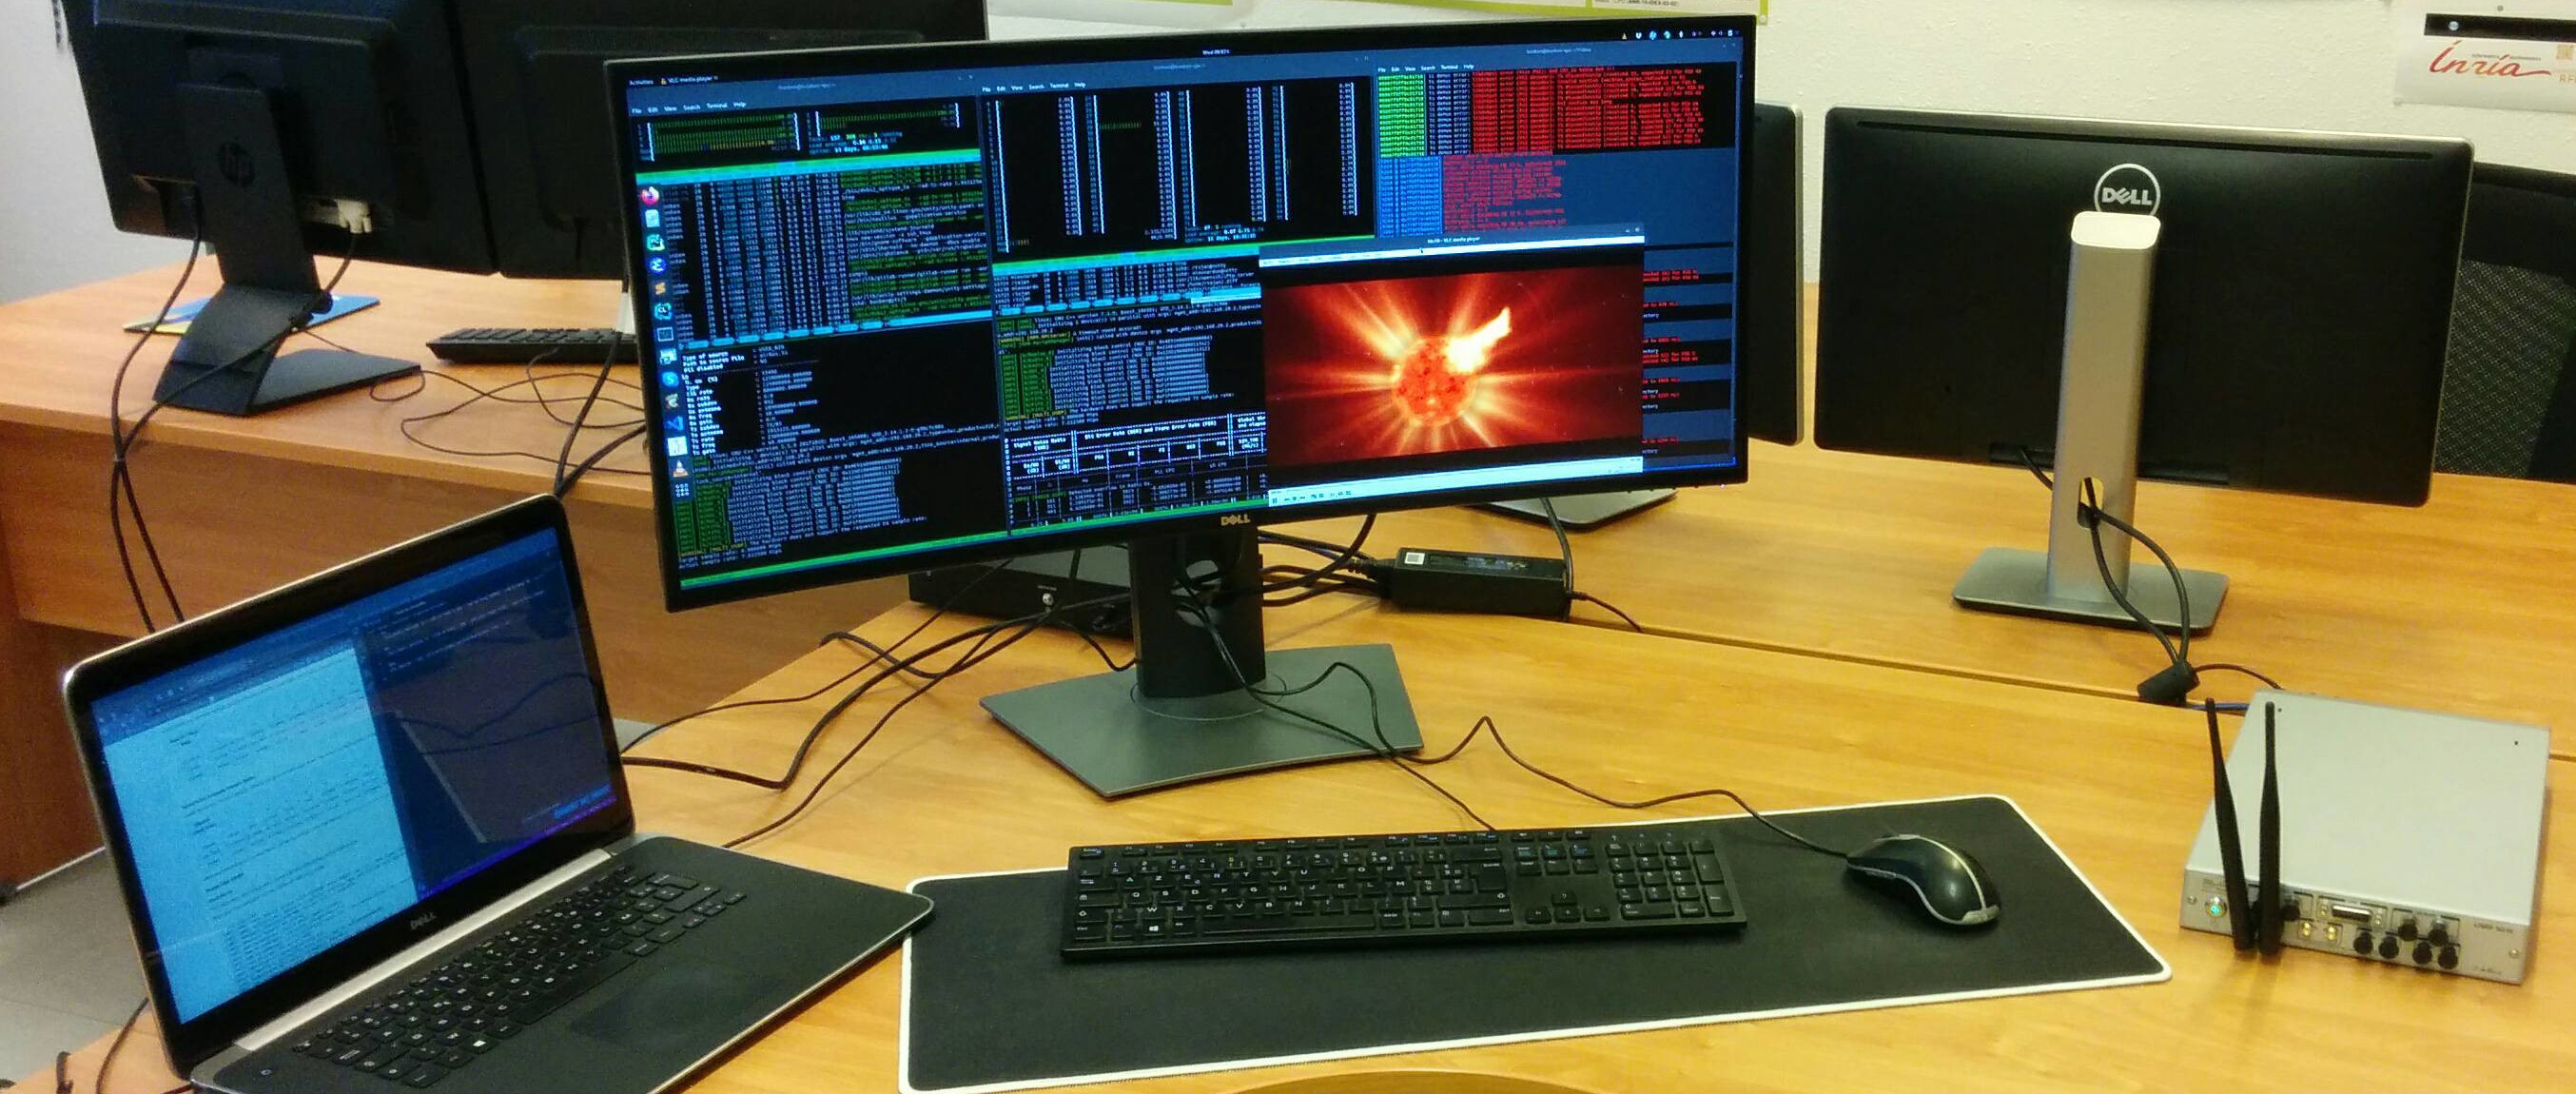
\includegraphics[scale=0.25]{pics/demo_dvbs2}
  % \end{figure}
  \vspace{+0.1cm}
  \begin{itemize}
    % \item Implement a full DVB-S2 transceiver (streaming video)
    \item<2-> 2x Universal Software Radio Peripherals (\textcolor{Paired-7}{USRPs}) N320 for the RF
    \item<3-> 1x Middle class computer for the digital transmitter (\textcolor{Paired-1}{Tx})
    \item<3-> 1x Server class computer for the digital receiver (\textcolor{Paired-3}{Rx})
    \item<5-> \textbf{Industrial constraint}: 30 $\sim$ 50 Mb/s
  \end{itemize}
  \vspace{-0.1cm}
  % \vfill
  \pause
  \pause
  \pause
  \begin{table}[htp]
    \centering
    \resizebox{1.0\linewidth}{!}{
    \begin{tabular}{c c c c c c c}
      \textbf{Config.} & \textbf{Modulation} & \textbf{Rate} $\bm{R}$ & $\bm{K_\text{\textbf{BCH}}}$ & $\bm{K_\text{\textbf{LDPC}}}$ & $\bm{N_\text{\textbf{LDPC}}}$ & $\bm{\mathcal{T}_i}$ (Rx, Seq.)\\
      \hline
      \textcolor{Paired-1}{MODCOD 1} &  QPSK & 3/5 &  9552 &  9720 & 16200 & 3.4 Mb/s\\
      \textcolor{Paired-3}{MODCOD 2} &  QPSK & 8/9 & 14232 & 14400 & 16200 & 4.1 Mb/s\\
      \textcolor{Paired-5}{MODCOD 3} & 8-PSK & 8/9 & 14232 & 14400 & 16200 & 4.0 Mb/s\\
    \end{tabular}
    }
    \caption*{Selected DVB-S2 configurations (MODCOD).}
  \end{table}
  % \vfill

\end{frame}

% \begin{frame}{Transmitter}
%   \vfill
%   \begin{figure}[!h]
%     \centering
%     \scalebox{.50}{
%     \begin{tikzpicture}%[scale=\tikzscale]
%       \tikzset{ tsk/.style ={draw=Paired-1, rounded corners=0pt, text=Paired-1, minimum height=1.0cm, minimum width=1cm} }
%       \tikzset{ stsk/.style={draw=Paired-1, rounded corners=0pt, text=Paired-1, minimum height=1.0cm, minimum width=1cm, fill=Paired-1!7} }
%       \tikzset{ ss/.style  ={draw=Paired-9, rounded corners=2pt, minimum height=1.5cm} }
%       \tikzset{ seq/.style ={draw=Paired-11, dashed, rounded corners=2pt} }
%       \tikzset{ mdl/.style ={draw=Paired-3,  dashed, rounded corners=2pt} }
%       \tikzset{ pip/.style ={draw=Dark2-8,  dotted, thick, rounded corners=2pt} }
%       \tikzset{ sin/.style ={draw=Paired-7, circle, minimum width=0.3cm, text=black, preaction={fill=white}, pattern=north east lines, pattern color=Paired-7} }
%       \tikzset{ sout/.style={draw=Paired-5, circle, minimum width=0.3cm, text=black, preaction={fill=white}, pattern=crosshatch dots, pattern color=Paired-5} }

%       \node[stsk                    , align=center] (t1) at (0.0, 2.0) {~generate~~\\($t^{\text{Tx}}_1$)};
%       \node[tsk , right=2.00cm of t1, align=center] (t2)               {~scramble~~\\($t^{\text{Tx}}_2$)};
%       \node[tsk , right=1.25cm of t2, align=center] (t3)               {~encode~~\\($t^{\text{Tx}}_3$)};
%       \node[tsk , right=1.25cm of t3, align=center] (t4)               {~encode~~\\($t^{\text{Tx}}_4$)};
%       \node[tsk , right=1.25cm of t4, align=center] (t5)               {~interleave~~\\($t^{\text{Tx}}_5$)};
%       \node[tsk,  below=1.00cm of t2, align=center] (t6)               {~modulate~~\\($t^{\text{Tx}}_6$)};
%       \node[tsk , right=1.25cm of t6, align=center] (t7)               {~insert~~\\($t^{\text{Tx}}_7$)};
%       \node[tsk , right=1.25cm of t7, align=center] (t8)               {~scramble~~\\($t^{\text{Tx}}_8$)};
%       \node[stsk, right=4.60cm of t8, align=center] (t9)               {~filter~~\\($t^{\text{Tx}}_9$)};
%       \node[stsk, right=1.00cm of t9, align=center] (t10)              {~send~~\\($t^{\text{Tx}}_{10}$)};

%       \node[sout, at=(t1.east) ] (t1_so)  {};
%       \node[sin,  at=(t2.west) ] (t2_si)  {};
%       \node[sout, at=(t2.east) ] (t2_so)  {};
%       \node[sin,  at=(t3.west) ] (t3_si)  {};
%       \node[sout, at=(t3.east) ] (t3_so)  {};
%       \node[sin,  at=(t4.west) ] (t4_si)  {};
%       \node[sout, at=(t4.east) ] (t4_so)  {};
%       \node[sin,  at=(t5.west) ] (t5_si)  {};
%       \node[sout, at=(t5.east) ] (t5_so)  {};
%       \node[sin,  at=(t6.west) ] (t6_si)  {};
%       \node[sout, at=(t6.east) ] (t6_so)  {};
%       \node[sin,  at=(t7.west) ] (t7_si)  {};
%       \node[sout, at=(t7.east) ] (t7_so)  {};
%       \node[sin,  at=(t8.west) ] (t8_si)  {};
%       \node[sout, at=(t8.east) ] (t8_so)  {};
%       \node[sin,  at=(t9.west) ] (t9_si)  {};
%       \node[sout, at=(t9.east) ] (t9_so)  {};
%       \node[sin,  at=(t10.west)] (t10_si) {};

%       \node[mdl, label={[Paired-3]above:Source Binary File},  fit=(t1)           (t1_so)] (m1) {};
%       \node[mdl, label={[Paired-3]above:Scrambler Binary},    fit=(t2)  (t2_si)  (t2_so)] (m2) {};
%       \node[mdl, label={[Paired-3]above:Encoder BCH},         fit=(t3)  (t3_si)  (t3_so)] (m3) {};
%       \node[mdl, label={[Paired-3]above:Encoder LDPC},        fit=(t4)  (t4_si)  (t4_so)] (m4) {};
%       \node[mdl, label={[Paired-3]above:Interleaver},         fit=(t5)  (t5_si)  (t5_so)] (m5) {};
%       \node[mdl, label={[Paired-3]above:Modem PSK},           fit=(t6)  (t6_si)  (t6_so)] (m6) {};
%       \node[mdl, label={[Paired-3]above:Framer PLH},          fit=(t7)  (t7_si)  (t7_so)] (m7) {};
%       \node[mdl, label={[Paired-3]above:Scrambler Symbol},    fit=(t8)  (t8_si)  (t8_so)] (m8) {};
%       \node[mdl, label={[Paired-3]above:Filter Shaping},      fit=(t9)  (t9_si)  (t9_so)] (m9) {};
%       \node[mdl, label={[Paired-3]above:Radio},               fit=(t10) (t10_si)        ] (m9) {};

%       \draw[->,>=latex] (t1_so) -- (t2_si)  node [midway, above] {};
%       \draw[->,>=latex] (t2_so) -- (t3_si)  node [midway, above] {};
%       \draw[->,>=latex] (t3_so) -- (t4_si)  node [midway, above] {};
%       \draw[->,>=latex] (t4_so) -- (t5_si)  node [midway, above] {};
%       \draw[->,>=latex] (t5_so) -- (13.9,2.0) -- (13.9,1.15) -- (2.25,1.15) -- (2.25,0) -- (t6_si)  node [midway, above] {};
%       \draw[->,>=latex] (t6_so) -- (t7_si)  node [midway, above] {};
%       \draw[->,>=latex] (t7_so) -- (t8_si)  node [midway, above] {};
%       \draw[->,>=latex] (t8_so) -- (t9_si)  node [midway, above] {};
%       \draw[->,>=latex] (t9_so) -- (t10_si) node [midway, above] {};
%       \draw[black, -] (t10.east)--++(0:1.0cm) node[antenna, label={[above,yshift=+2.15cm]USRP}] {};

%       \node[seq, minimum height=2.5cm, minimum width=3.5cm,  label={[Paired-11]below:Stage 1}, fit=(t1) (t1_so)                                      ] (seq1) {};
%       \node[seq, minimum height=4.5cm, minimum width=12.0cm, label={[Paired-11]below:Stage 2}, fit=(t2_si) (t2) (t3) (t4) (t5) (t6) (t7) (t8) (t8_so)] (seq2) {};
%       \node[seq, minimum height=2.5cm, minimum width=4.5cm,  label={[Paired-11]below:Stage 3}, fit=(t9_si) (t10)                                     ] (seq3) {};
%     \end{tikzpicture}
%     }
%   \end{figure}
%   \vfill
% \end{frame}

\begin{frame}{Receiver (Rx)}
  \vspace{-0.3cm}
  \begin{figure}[!h]
    \centering
    \scalebox{.40}{
    \begin{tikzpicture}%[scale=\tikzscale]
      \tikzset{ tsk/.style ={draw=Paired-1, rounded corners=0pt, text=Paired-1, minimum height=1.0cm, minimum width=1cm} }
      \tikzset{ stsk/.style={draw=Paired-1, rounded corners=0pt, text=Paired-1, minimum height=1.0cm, minimum width=1cm, fill=Paired-1!7} }
      \tikzset{ ss/.style  ={draw=Paired-9, rounded corners=2pt, minimum height=1.5cm} }
      \tikzset{ seq/.style ={draw=Paired-11, dashed, rounded corners=2pt} }
      \tikzset{ mdl/.style ={draw=Paired-3,  dashed, rounded corners=2pt} }
      \tikzset{ pip/.style ={draw=Dark2-8,  dotted, thick, rounded corners=2pt} }
      \tikzset{ sin/.style ={draw=Paired-7, circle, minimum width=0.3cm, text=black, preaction={fill=white}, pattern=north east lines, pattern color=Paired-7} }
      \tikzset{ sout/.style={draw=Paired-5, circle, minimum width=0.3cm, text=black, preaction={fill=white}, pattern=crosshatch dots, pattern color=Paired-5} }

      \node[stsk                     , align=center] (t1) at ( 0.0, 2.0) {~receive~~\\($t^{\text{Rx}}_1$)};
      \node[tsk , right=2.00cm of t1 , align=center] (t2)                {~imultiply~~\\($t^{\text{Rx}}_2$)};
      \node[stsk, right=1.00cm of t2 , align=center] (t3)                {~synchronize~~\\($t^{\text{Rx}}_3$)};
      \node[stsk, right=1.00cm of t3 , align=center] (t4)                {~filter~~\\($t^{\text{Rx}}_4$)};
      \node[stsk, below=3.50cm of t2 , align=center] (t5)                {~synchronize~~\\($t^{\text{Rx}}_5$)};
      \node[stsk, right=2.00cm of t5 , align=center] (t6)                {~extract~~\\($t^{\text{Rx}}_6$)};
      \node[tsk , right=1.00cm of t6 , align=center] (t7)                {~imultiply~~\\($t^{\text{Rx}}_7$)};
      \node[stsk, right=1.00cm of t7 , align=center] (t8)                {~synchronize~~\\($t^{\text{Rx}}_8$)};
      \node[tsk , below=3.50cm of t5 , align=center] (t9)                {~descramble~~\\($t^{\text{Rx}}_9$)};
      \node[stsk, right=1.00cm of t9 , align=center] (t10)               {~synchronize~~\\($t^{\text{Rx}}_{10}$)};
      \node[tsk , right=1.00cm of t10, align=center] (t11)               {~synchronize~~\\($t^{\text{Rx}}_{11}$)};
      \node[tsk , right=3.00cm of t11, align=center] (t12)               {~remove~~\\($t^{\text{Rx}}_{12}$)};
      \node[tsk , right=1.00cm of t12, align=center] (t13)               {~estimate~~\\($t^{\text{Rx}}_{13}$)};
      \node[tsk , below=3.50cm of t9 , align=center] (t14)               {~demodulate~~\\($t^{\text{Rx}}_{14}$)};
      \node[tsk , right=1.00cm of t14, align=center] (t15)               {~deinterleave~~\\($t^{\text{Rx}}_{15}$)};
      \node[tsk , right=1.00cm of t15, align=center] (t16)               {~decode SIHO~~\\($t^{\text{Rx}}_{16}$)};
      \node[tsk , right=1.00cm of t16, align=center] (t17)               {~decode HIHO~~\\($t^{\text{Rx}}_{17}$)};
      \node[tsk , right=1.00cm of t17, align=center] (t18)               {~descramble~~\\($t^{\text{Rx}}_{18}$)};
      \node[stsk, right=2.00cm of t18, align=center] (t19)               {~send~~\\($t^{\text{Rx}}_{19}$)};

      \node[sout, at=(t1.east)                ] (t1_so)  {};
      \node[sin,  at=(t2.west)                ] (t2_si)  {};
      \node[sout, at=(t2.east)                ] (t2_so)  {};
      \node[sin,  at=(t3.west)                ] (t3_si)  {};
      \node[sout, at=(t3.east)                ] (t3_so)  {};
      \node[sin,  at=(t4.west)                ] (t4_si)  {};
      \node[sout, at=(t4.east)                ] (t4_so)  {};
      \node[sin,  at=(t5.west)                ] (t5_si)  {};
      \node[sout, at=(t5.east), yshift=+0.25cm] (t5_so1) {};
      \node[sout, at=(t5.east), yshift=-0.25cm] (t5_so2) {};
      \node[sin,  at=(t6.west), yshift=+0.25cm] (t6_si1) {};
      \node[sin,  at=(t6.west), yshift=-0.25cm] (t6_si2) {};
      \node[sout, at=(t6.east)                ] (t6_so)  {};
      \node[sin,  at=(t7.west)                ] (t7_si)  {};
      \node[sout, at=(t7.east)                ] (t7_so)  {};
      \node[sin,  at=(t8.west)                ] (t8_si)  {};
      \node[sout, at=(t8.east), yshift=+0.25cm] (t8_so1) {};
      \node[sout, at=(t8.east), yshift=-0.25cm] (t8_so2) {};
      \node[sin,  at=(t9.west)                ] (t9_si)  {};
      \node[sout, at=(t9.east)                ] (t9_so)  {};
      \node[sin,  at=(t10.west)               ] (t10_si) {};
      \node[sout, at=(t10.east)               ] (t10_so) {};
      \node[sin,  at=(t11.west)               ] (t11_si) {};
      \node[sout, at=(t11.east)               ] (t11_so) {};
      \node[sin,  at=(t12.west)               ] (t12_si) {};
      \node[sout, at=(t12.east)               ] (t12_so) {};
      \node[sin,  at=(t13.west)               ] (t13_si) {};
      \node[sout, at=(t13.east)               ] (t13_so) {};
      \node[sin,  at=(t14.west)               ] (t14_si) {};
      \node[sout, at=(t14.east)               ] (t14_so) {};
      \node[sin,  at=(t15.west)               ] (t15_si) {};
      \node[sout, at=(t15.east)               ] (t15_so) {};
      \node[sin,  at=(t16.west)               ] (t16_si) {};
      \node[sout, at=(t16.east)               ] (t16_so) {};
      \node[sin,  at=(t17.west)               ] (t17_si) {};
      \node[sout, at=(t17.east)               ] (t17_so) {};
      \node[sin,  at=(t18.west)               ] (t18_si) {};
      \node[sout, at=(t18.east)               ] (t18_so) {};
      \node[sin,  at=(t19.west)               ] (t19_si) {};

      \draw[black, -] (t1.west)--++(0:-1.0cm) node[antenna, label={[above,yshift=+2.15cm,Paired-7]USRP}] {};
      \draw[->,>=latex] (t1_so) -- (t2_si)  node [midway, above] {};
      \draw[->,>=latex] (t2_so) -- (t3_si)  node [midway, above] {};
      \draw[->,>=latex] (t3_so) -- (t4_si)  node [midway, above] {};
      % \draw[->,>=latex] (t4_so) -- (t5_si)  node [midway, above] {};
      \draw[->,>=latex] (t4_so) -| (11.0,-0.5) -- (1.5,-0.5) |- (t5_si)  node [midway, above] {};
      \draw[->,>=latex] (t5_so1) -- (t6_si1)  node [midway, above] {};
      \draw[->,>=latex] (t5_so2) -- (t6_si2)  node [midway, above] {};
      % \draw[->,>=latex] (t5_so) -- (13.9,2.0) -- (13.9,1.15) -- (2.25,1.15) -- (2.25,0) -- (t6_si)  node [midway, above] {};
      \draw[->,>=latex] (t6_so) -- (t7_si)  node [midway, above] {};
      \draw[->,>=latex] (t7_so) -- (t8_si)  node [midway, above] {};
      % \draw[->,>=latex] (t8_so) -- (t9_si)  node [midway, above] {};
      \draw[->,>=latex] (t8_so1) -| (15.5,-5.0) -- (1.5,-5.0) |- (t9_si)  node [midway, above] {};
      \draw[->,>=latex] (t9_so) -- (t10_si) node [midway, above] {};
      \draw[->,>=latex] (t10_so) -- (t11_si) node [midway, above] {};
      \draw[->,>=latex] (t11_so) -- (t12_si) node [midway, above] {};
      \draw[->,>=latex] (t12_so) -- (t13_si) node [midway, above] {};
      % \draw[->,>=latex] (t13_so) -- (t14_si) node [midway, above] {};
      \draw[->,>=latex] (t13_so) -| (19.5,-9.5) -- (1.5,-9.5) |- (t14_si)  node [midway, above] {};

      \draw[->,>=latex] (t14_so) -- (t15_si) node [midway, above] {};
      \draw[->,>=latex] (t15_so) -- (t16_si) node [midway, above] {};
      \draw[->,>=latex] (t16_so) -- (t17_si) node [midway, above] {};
      \draw[->,>=latex] (t17_so) -- (t18_si) node [midway, above] {};
      \draw[->,>=latex] (t18_so) -- (t19_si) node [midway, above] {};

      \node[seq, minimum height=3.5cm, minimum width=3.2cm,   label={[Paired-11]below:Stage 1}, fit=(t1)  (t1_so)                                                          ] (seq1) {};
      \node[seq, minimum height=3.5cm, minimum width=8.5cm,   label={[Paired-11]below:Stage 2}, fit=(t2)  (t2_si)  (t2_so)  (t3)  (t3_si)  (t3_so)  (t4)  (t4_si)  (t4_so) ] (seq2) {};
      \only<1-3>{
      \node[seq, minimum height=3.5cm, minimum width=3.5cm,   label={[Paired-11]below:Stage 3}, fit=(t5)  (t5_si)  (t5_so1)                                                ] (seq3) {};
      }
      \only<4->{
      \node[seq, minimum height=3.5cm, minimum width=3.5cm,   label={[Paired-11]below:Stage 3}, fit=(t5)  (t5_si)  (t5_so1), line width=1.0mm                              ] (seq3) {};
      }
      \node[seq, minimum height=3.5cm, minimum width=9.0cm,   label={[Paired-11]below:Stage 4}, fit=(t6)  (t6_si1) (t6_so)  (t7)  (t7_si)  (t7_so)  (t8)  (t8_si)  (t8_so1)] (seq4) {};
      \node[seq, minimum height=3.5cm, minimum width=10.0cm,  label={[Paired-11]below:Stage 5}, fit=(t9)  (t9_si)  (t9_so)  (t10) (t10_si) (t10_so) (t11) (t11_si) (t11_so)] (seq5) {};
      \node[seq, minimum height=3.5cm, minimum width=6.5cm,   label={[Paired-11]below:Stage 6}, fit=(t12) (t12_si) (t12_so) (t13) (t13_si) (t13_so)                        ] (seq6) {};
      \only<1>{
      \node[seq, minimum height=3.5cm, minimum width=17.0cm,  label={[Paired-11]below:Stage 7}, fit=(t14_si) (t18_so)                                                      ] (seq7) {};
      }
      \only<2>{
      \node[seq, minimum height=3.5cm, minimum width=17.0cm,  label={[Paired-11]below:Stage 7}, fit=(t14_si) (t18_so), line width=1.0mm                                               ] (seq7) {};
      }
      \only<3->{
      \node[seq, minimum height=3.5cm, minimum width=17.0cm,  label={[Paired-11]below:Stage 7 (\textbf{parallelized on 28 cores} with the sequence duplication technique)}, fit=(t14_si) (t18_so)                                                      ] (seq7) {};
      }
      \node[seq, minimum height=3.5cm, minimum width=3.2cm,   label={[Paired-11]below:Stage 8}, fit=(t19_si) (t19)                                                         ] (seq8) {};

      \node[mdl, label={[Paired-3, align=center]above:Radio},                          fit=(t1)           (t1_so)     ] (m1)  {};
      \node[mdl, label={[Paired-3, align=center]above:Multiplier AGC},                 fit=(t2)  (t2_si)  (t2_so)     ] (m2)  {};
      \node[mdl, label={[Paired-3, align=center]above:Synchronizer\\Freq. Coarse},     fit=(t3)  (t3_si)  (t3_so)     ] (m3)  {};
      \node[mdl, label={[Paired-3, align=center]above:Filter\\Matched},                fit=(t4)  (t4_si)  (t4_so)     ] (m4)  {};
      \node[mdl, label={[Paired-3, align=center]above:Synchronizer Timing\\(Gardner)}, fit=(t5)  (t5_si)  (t6) (t6_so)] (m5)  {};
      \node[mdl, label={[Paired-3, align=center]above:Multiplier AGC},                 fit=(t7)  (t7_si)  (t7_so)     ] (m6)  {};
      \node[mdl, label={[Paired-3, align=center]above:Synchronizer\\Frame},            fit=(t8)  (t8_si)  (t8_so1)    ] (m7)  {};
      \node[mdl, label={[Paired-3, align=center]above:Scrambler Symbol},               fit=(t9)  (t9_si)  (t9_so)     ] (m8)  {};
      \node[mdl, label={[Paired-3, align=center]above:Synchronizer\\Freq. Fine L\&R},  fit=(t10) (t10_si) (t10_so)    ] (m9)  {};
      \node[mdl, label={[Paired-3, align=center]above:Synchronizer\\Freq. Fine P/F},   fit=(t11) (t11_si) (t11_so)    ] (m10) {};
      \node[mdl, label={[Paired-3, align=center]above:Framer PLH},                     fit=(t12) (t12_si) (t12_so)    ] (m11) {};
      \node[mdl, label={[Paired-3, align=center]above:Noise Estimator},                fit=(t13) (t13_si) (t13_so)    ] (m12) {};
      \node[mdl, label={[Paired-3, align=center]above:Modem PSK},                      fit=(t14) (t14_si) (t14_so)    ] (m13) {};
      \node[mdl, label={[Paired-3, align=center]above:Interleaver},                    fit=(t15) (t15_si) (t15_so)    ] (m14) {};
      \node[mdl, label={[Paired-3, align=center]above:Decoder LDPC},                   fit=(t16) (t16_si) (t16_so)    ] (m15) {};
      \node[mdl, label={[Paired-3, align=center]above:Decoder BCH},                    fit=(t17) (t17_si) (t17_so)    ] (m16) {};
      \node[mdl, label={[Paired-3, align=center]above:Scrambler Binary},               fit=(t18) (t18_si) (t18_so)    ] (m17) {};
      \node[mdl, label={[Paired-3, align=center]above:Sink Binary File},               fit=(t19) (t19_si)             ] (m18) {};
    \end{tikzpicture}
    }
  \end{figure}
\end{frame}

\begin{frame}{Evaluation}
  \vspace{-0.5cm}
  \begin{columns}
  \begin{column}[T]{6cm}
  \begin{figure}[!h]
    \centering
    \scalebox{.50}{
    \begin{tikzpicture}%[scale=\tikzscale]
    \begin{axis}[/pgfplots/table/ignore chars={|}, %footnotesize,
                      height=1.54\textwidth, width=2.0\textwidth,
                      xticklabel style={black!70}, yticklabel style={black!70},
                      ymode = log,
                      ylabel=Frame Error Rate,
                      % ymin=0.000000001, ymax=0.05,
                      % xmin=0, xmax=2,
                      % xtick={0,0.5,...,4.5},
                      xlabel=$E_b/N_0~\text{(dB)}$,
                      grid=both, grid style={gray!30},
                      %tick align=outside, tickpos=left,
                      legend pos=north east]
      \addplot[mark=square,    Paired-1!60, semithick, mark options={solid}] table [x=Eb/N0, y=FER] {../main/chapter5/fig/dvbs2/bfer/dat/data_QPSK_R_3_5_BB.txt};  \label{plot:llline1}
      \addplot[mark=o,         Paired-1,    semithick, mark options={solid}, domain=0:0.2, error bars/.cd, x dir=both,x fixed=0.2, y dir=both,y explicit, error bar style={solid}] table [x=Eb/N0, y=FER] {../main/chapter5/fig/dvbs2/bfer/dat/data_QPSK_R_3_5_rad.txt}; \label{plot:llline3}
      \addplot[mark=square,    Paired-3!60, semithick, mark options={solid}] table [x=Eb/N0, y=FER] {../main/chapter5/fig/dvbs2/bfer/dat/data_QPSK_R_8_9_BB.txt};  \label{plot:llline4}
      \addplot[mark=o,         Paired-3,    semithick, mark options={solid}, domain=0:0.2, error bars/.cd, x dir=both,x fixed=0.2, y dir=both,y explicit, error bar style={solid}] table [x=Eb/N0, y=FER] {../main/chapter5/fig/dvbs2/bfer/dat/data_QPSK_R_8_9_rad.txt}; \label{plot:llline6}
      \addplot[mark=square,    Paired-5!60, semithick, mark options={solid}] table [x=Eb/N0, y=FER] {../main/chapter5/fig/dvbs2/bfer/dat/data_8PSK_R_8_9_BB.txt};  \label{plot:llline7}
      \addplot[mark=o,         Paired-5,    semithick, mark options={solid}, domain=0:0.2, error bars/.cd, x dir=both,x fixed=0.2, y dir=both,y explicit, error bar style={solid}] table [x=Eb/N0, y=FER] {../main/chapter5/fig/dvbs2/bfer/dat/data_8PSK_R_8_9_rad.txt}; \label{plot:llline9}
      \coordinate (legend) at (axis description cs:0.875,1.05);
    \end{axis}

    \matrix [
        draw,
        matrix of nodes,
        anchor=south east,
        fill=white,
        ampersand replacement=\&
    ] at (legend) {
                 \& \textcolor{Paired-1}{MODCOD 1} \& \textcolor{Paired-3}{MODCOD 2} \& \textcolor{Paired-5}{MODCOD 3} \\
        AWGN     \& \ref{plot:llline1} \& \ref{plot:llline4} \& \ref{plot:llline7} \\
        % AWGN$^+$ \& \ref{plot:llline2} \& \ref{plot:llline5} \& \ref{plot:llline8} \\
        Real     \& \ref{plot:llline3} \& \ref{plot:llline6} \& \ref{plot:llline9} \\
    };
    \end{tikzpicture}
    }
  \end{figure}
  \end{column}
  \begin{column}[T]{6cm}
    \vspace{1.7cm}
    \begin{table}[htp]
    \centering
    % \caption
    %   [Throughput performance depending of the selected DVB-S2 configuration.]
    %   {Throughput performance depending of the selected DVB-S2 configuration.}
    % \label{tab:sdr_dvbs2_thr_modcod}
    {\small\resizebox{1.0\linewidth}{!}{
    \begin{tabular}{c | c | c }
      \multirow{2}{*}{\textbf{Config.}} & \multicolumn{2}{c }{\textbf{Throughput} $\bm{\mathcal{T}_i}$ (Mb/s)} \\
                                        & \multicolumn{1}{c |}{\textbf{Sequential}} & \multicolumn{1}{c }{\textbf{Parallel}} \\
      \hline
      \textcolor{Paired-1}{MODCOD 1} & 3.4 & 37 \\
      \textcolor{Paired-3}{MODCOD 2} & 4.1 & 55 \\
      \textcolor{Paired-5}{MODCOD 3} & 4.0 & 80 \\
    \end{tabular}
    }}
  \end{table}
  \end{column}
  \end{columns}

  \begin{itemize}
    \item<2-> \textbf{Full SDR system} compatible with industrial constraints
    \item<3-> \textbf{Speedups from 10 to 20} thanks to the proposed \AFFECT eDSL
    \item<4-> Support of \textbf{3 different configurations} {\color{bleuUni}\Large\MVRightarrow} \textbf{Software flexibility}
  \end{itemize}

\end{frame}
